\section{Shape and Palette comparisons}
\label{app:variants}

The main paper focuses on Color. Shape and Palette repeat the same routing
problem with triangles/diamonds and green/blue cues, respectively. They show
the same qualitative ordering: location coordinates are easier to recover
than cue-indexed coordinates, and planning is less successful when the
correct entrance is farther away. The values differ across variants; these
single-model comparisons do not establish statistical equivalence.

Tables~\ref{tab:variantprobes} and \ref{tab:variantrankplanning} retain the
complete results, including Color as a reference. Linear location $R^2$
averages .907 and .930 for Shape and Palette, versus .203 and .258 for cue
coordinates. The MLP preserves this gap. Decoder and landscape comparisons
appear in Figures~\ref{fig:variant-decoders} and
\ref{fig:variant-landscapes-swaps}. The quantitative landscape protocol is in
Appendix~\ref{app:landscapes}; Appendix~\ref{app:portal-swap} gives the full
swap controls and uncertainty. Source revisions and decoder snapshot times
differ, as detailed in Appendix~\ref{app:planning}.

\begin{table}[!htbp]
\centering
\caption{\textbf{Linear and MLP probes recover locations more accurately than cues.} Entries are linear/MLP MAE (pixels) and $R^2$, averaged over $x/y$; MLP values average three fits. Top/bottom are ordered within each room group; cue rows identify paired endpoints. Both use the same test episodes, with 640/512 fit episodes (Appendix~\ref{app:nonlinear}).}
\label{tab:variantprobes}
\renewcommand{\arraystretch}{1.10}
\setlength{\tabcolsep}{3pt}
\begin{tabular*}{\linewidth}{@{\extracolsep{\fill}}llrrrr@{}}
\toprule
 & & \multicolumn{2}{c}{Central room} & \multicolumn{2}{c}{Destination rooms} \\
\cmidrule(lr){3-4}\cmidrule(l){5-6}
Variant & Endpoint & MAE $\downarrow$ & $R^2\uparrow$ & MAE $\downarrow$ & $R^2\uparrow$ \\
\midrule
Color & Top & \curpred{4.63}{6.14} & \curpred{.919}{.851} & \curpred{2.72}{3.82} & \curpred{.960}{.925} \\
 & Bottom & \curpred{5.14}{6.34} & \curpred{.900}{.844} & \curpred{2.82}{4.06} & \curpred{.958}{.919} \\
\noalign{\vskip 2pt}
\cdashline{2-6}[.5pt/2pt]
\noalign{\vskip 2pt}
 & Green & \curpred{25.05}{25.43} & \curpred{.256}{.275} & \curpred{29.81}{29.47} & \curpred{.180}{.257} \\
 & Orange & \curpred{25.01}{25.40} & \curpred{.289}{.318} & \curpred{29.72}{29.72} & \curpred{.172}{.240} \\
\midrule
Shape & Top & \curpred{5.88}{7.27} & \curpred{.868}{.803} & \curpred{3.19}{4.32} & \curpred{.941}{.905} \\
 & Bottom & \curpred{6.06}{7.28} & \curpred{.872}{.809} & \curpred{3.14}{4.16} & \curpred{.948}{.911} \\
\noalign{\vskip 2pt}
\cdashline{2-6}[.5pt/2pt]
\noalign{\vskip 2pt}
 & Triangle & \curpred{25.18}{25.36} & \curpred{.229}{.284} & \curpred{30.75}{29.91} & \curpred{.144}{.207} \\
 & Diamond & \curpred{25.80}{25.76} & \curpred{.253}{.310} & \curpred{30.47}{29.95} & \curpred{.184}{.241} \\
\midrule
Palette & Top & \curpred{4.79}{6.56} & \curpred{.913}{.830} & \curpred{2.63}{3.68} & \curpred{.962}{.929} \\
 & Bottom & \curpred{5.34}{7.00} & \curpred{.893}{.821} & \curpred{2.96}{4.04} & \curpred{.952}{.915} \\
\noalign{\vskip 2pt}
\cdashline{2-6}[.5pt/2pt]
\noalign{\vskip 2pt}
 & Green & \curpred{24.93}{25.80} & \curpred{.262}{.265} & \curpred{29.06}{30.00} & \curpred{.217}{.211} \\
 & Blue & \curpred{24.95}{25.89} & \curpred{.315}{.303} & \curpred{28.88}{29.44} & \curpred{.239}{.257} \\
\bottomrule
\end{tabular*}
\end{table}

\begin{table}[!htbp]
\centering
\caption{\textbf{Planning success separates more clearly by rank than by cue.}
Entries show CEM/GD task success (\%). Cue 1/Cue 2 denote green/orange (Color),
triangle/diamond (Shape), and green/blue (Palette).
R1/R2 have 25 cases each; Cue 1/Cue 2 have 16/34 cases, pooling both ranks.
Appendix~\ref{app:planning} gives the full cue-by-rank breakdown.}
\label{tab:variantrankplanning}
\renewcommand{\arraystretch}{1.12}
\begin{tabular*}{\linewidth}{@{\extracolsep{\fill}}lcccc@{}}
\toprule
Variant & \multicolumn{2}{c}{Rank-based performance $\uparrow$} & \multicolumn{2}{c}{Cue-based performance $\uparrow$} \\
\cmidrule(lr){2-3}\cmidrule(l){4-5}
 & R1 & R2 & Cue 1 & Cue 2 \\
\midrule
Color & 80/64 & 16/52 & 56.3/62.5 & 44.1/55.9 \\
Shape & 88/76 & 24/40 & 68.8/56.3 & 50.0/58.8 \\
Palette & 80/84 & 28/32 & 56.3/75.0 & 52.9/50.0 \\
\bottomrule
\end{tabular*}
\end{table}

\begin{figure}[H]
  \centering
  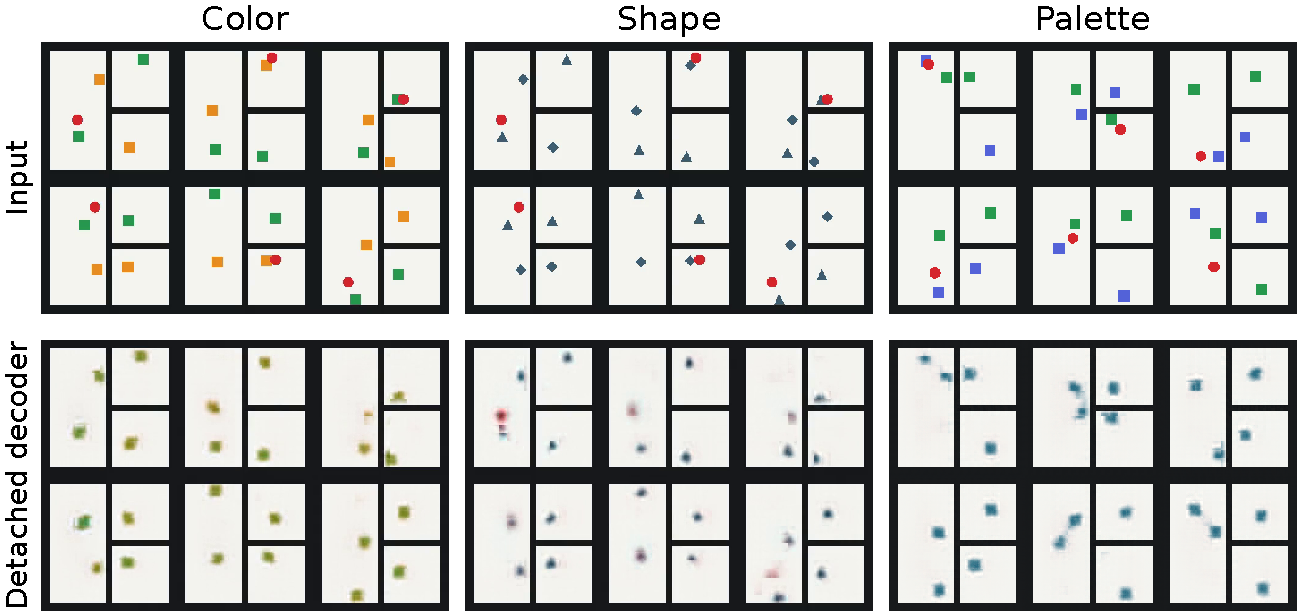
\includegraphics[width=\linewidth]{figures/lewm_spatial_three_cue_decoders.pdf}
  \caption{\textbf{Reconstructions preserve the rooms but weaken their cues.}
  Original observations (top) and decoded images (bottom) for Color, Shape,
  and Palette. All six recorded clips per variant are shown. Snapshot
  timing and the decoder protocol are given in
  Appendix~\ref{app:planning}.}
  \label{fig:variant-decoders}
\end{figure}

\begin{figure}[H]
  \centering
  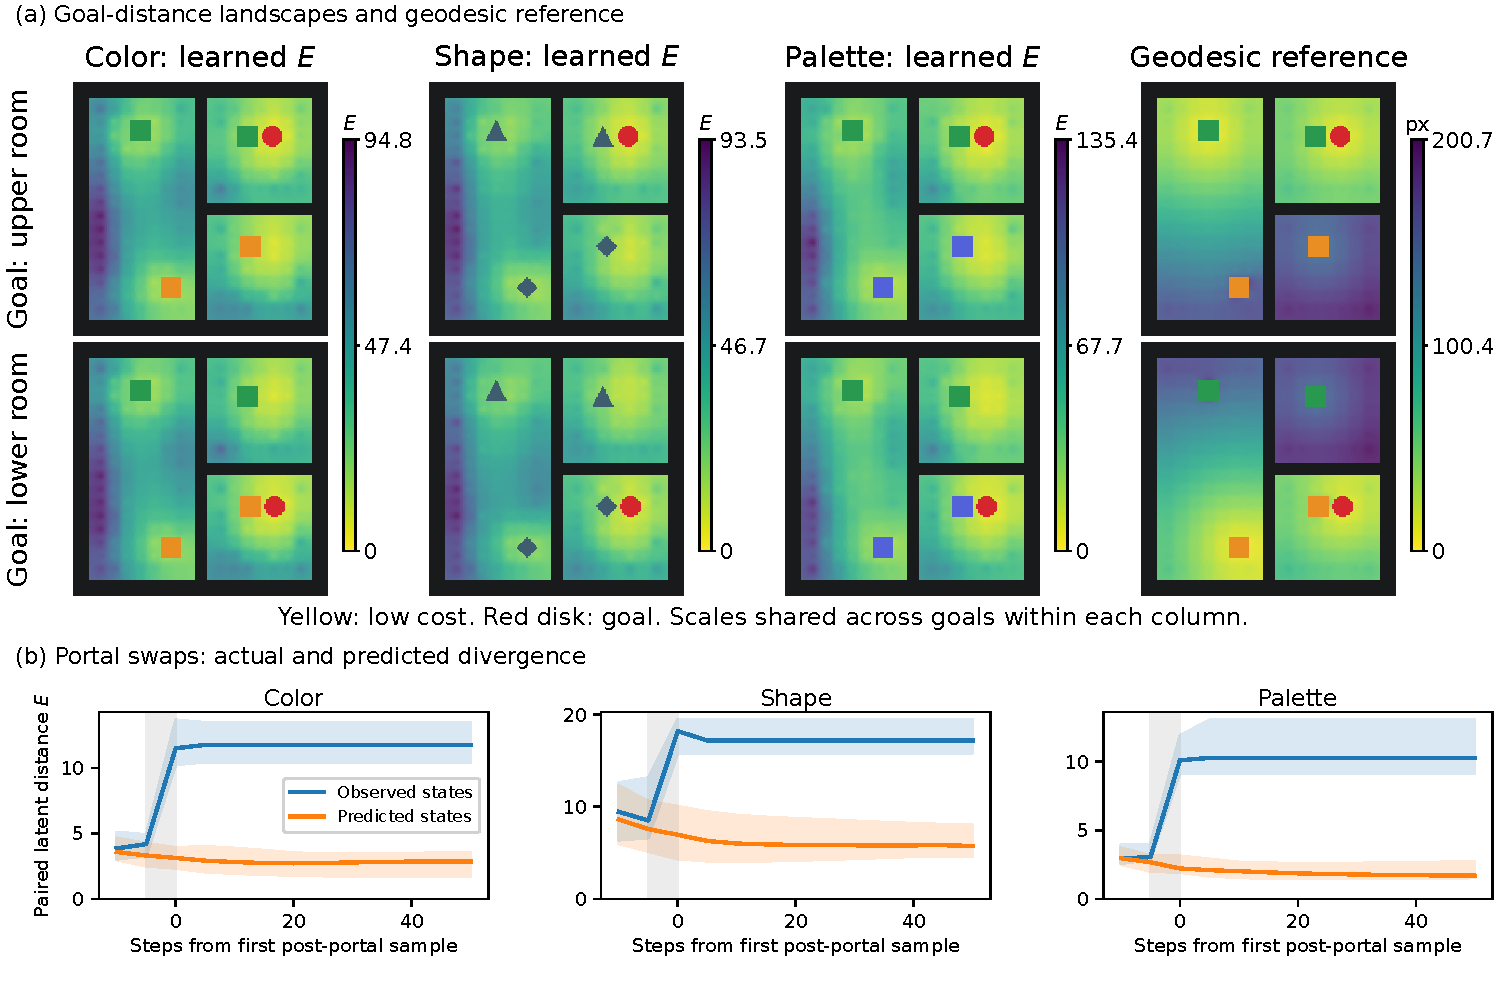
\includegraphics[width=\linewidth]{figures/lewm_goal_landscape_and_portal_swap.pdf}
  \caption{\textbf{Goal similarity and predicted dynamics both weaken route distinctions.}
  (a) LeWM goal energies and geodesic distance; rows switch the goal room.
  Yellow denotes low cost; red disks mark goals. Each column shares a scale across goals;
  latent energy and travel distance have different units.
  (b) Cue swaps: squared distance between the two worlds' encoded observations (blue)
  or model rollouts (orange). Early rollout values include conditioning observations.
  Medians and interquartile bands cover the same 16 geometries at every step.
  The gray interval contains teleportation. Latent scales differ across models.}
  \label{fig:variant-landscapes-swaps}
\end{figure}
